%==============================================================================
% @author Clinton Freeman
% @date 12/18/2013
%==============================================================================

\documentclass[oneside]{memoir}   

\usepackage{rc_style} 

\begin{document} 

%==============================================================================
% Cover page
%==============================================================================
   
\frontmatter

%\pagecolor{answerColor}
%\color{white}

\pagenumbering{gobble}
\thispagestyle{empty}     

%\begin{mdframed}[style=answer]  
\noindent{\fontsize{48pt}{64pt}\myfont\selectfont Rational\textbf{CAD} 0.1}
    
\vspace{1.5em}   

\noindent{\fontsize{24pt}{48pt}\myfont\selectfont User Manual}
%\end{mdframed}   
%\vspace{10em}  
\par\vspace*{\fill}

%\noindent\hfill{\fontsize{16pt}{24pt}\selectfont by CLINTON FREEMAN}  

\clearpage
 
%\pagecolor{white}   
%\color{black}

%\newpage\null\thispagestyle{empty}\newpage  

%==============================================================================
% Table of Contents 
%==============================================================================

\pagenumbering{roman}

\begingroup
\hypersetup{linkcolor=black}
\tableofcontents*
\endgroup   
 
\clearpage

%==============================================================================
% Preface
%==============================================================================

% \chapter{Preface}  
% 
% I am writing this book because I have yet to find a single source that clearly
% outlines what is to be done about geometric nonrobustness from both a
% theoretical and practical point of view.
% 
% \vspace{2em}
% \hfill\textbf{Clinton Freeman}
% 
% \hfill\textit{Chapel Hill, North Carolina}
% 
% \hfill January 2014

%==============================================================================
% Introduction
%==============================================================================

\mainmatter   
\pagenumbering{arabic}
     
\chapterstyle{freeman}

\chapter{Introduction}         
 
\chapterprecishere{``Begin at the beginning,� the King said gravely, ``and go on
 till you come to the end: then stop."\par\raggedleft--- \textup{Lewis Carroll}, Alice in Wonderland}

%\epigraph{``Begin at the beginning," the King said gravely, ``and go on till
% you come to the end: then stop."}{--- \textup{Lewis Carroll}, Alice in Wonderland}
 

%\section{Audience}    
 
Thanks for trying out RationalCAD, the simplest, easiest way to create robust
geometric models with convex polyhedra. This document describes what RationalCAD
is, how it differs from other editors, and how to use its powerful features to
create works of art.
 
\section{Interface Overview}
 
\begin{figure}[h!]
  \centering
    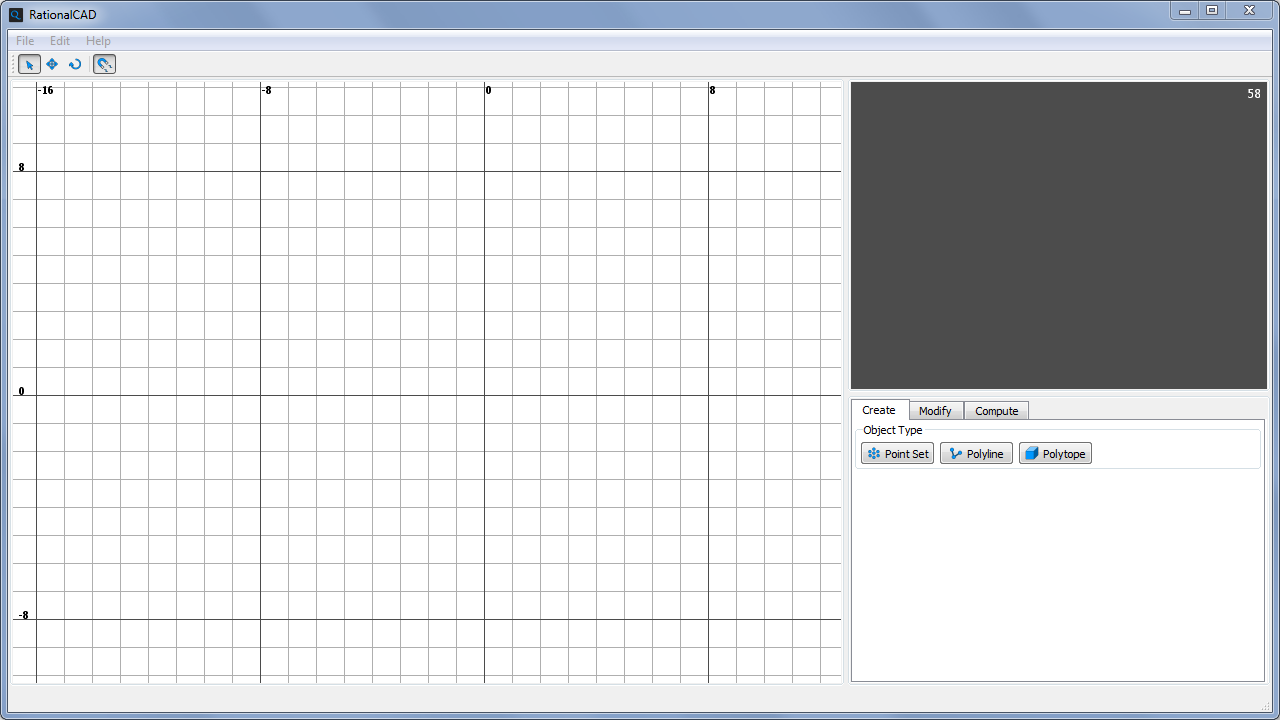
\includegraphics[width=0.9\textwidth]{images/interface-overview}
\end{figure}

The Graphical User Interface (GUI) comprises 7 components: the menubar, the
toolbar, the orthographic widget, the perspective widget, the interactive panel,
the statusbar, and the console.

% ![GUI Overview](http://cs.unc.edu/~freeman/DDAD/media/gui-overview.png)
\paragraph{Menubar.} The menubar comprises 3 high-level menus: File, Edit, and
Help. It exists primarily as a scaffold for future functionality.

\begin{itemize}
	\item File. The File menu is currently empty but
	\href{https://github.com/unc-compgeom/DDAD/issues/6}{issue $\triangle$ 6}
	specifies saving and loading of files. To do this, we need a mechanism for
	serializing and deserializing the scene, which is a major undertaking.
    \item Edit. The Edit menu contains one element, Preferences (there are
    issues to add duplicating and copy/paste.) Clicking Preferences will open a
    dialog which is split into 3 major panels. On the left is a list of
    subsections. The list currently contains only Grid Settings. On the right is
    a detailed view of the selected subsection. This detail view is
    parameterized by the list on the left. Finally, the bottom contains 4
    buttons: Default, Cancel, Apply, and Ok. The most interesting of these is
    Default, which requires the application to somehow define defaults. Settings
    \& Defaults bring up the notion of a configuration file (e.g. .ini). While
    currently there are not many settings, the dialog sets forth a framework
    into which developers can add new configurations settings.
    \item Help. The Help menu contains two simple elements. The first is a link
    to the user manual (the wiki). The second is an About dialog that provides
    information about the program version and a link to the project webpage.
\end{itemize}

\paragraph{Toolbar.} The toolbar comprises 4 elements: 3 buttons to control
input mode (Select, Translate, and Rotate), and 1 button to toggle snapping to
grid. The three input mode buttons are mutually exclusive with one another and
with the creation buttons in the interactive panel. The select mode is initially
activated and allows the user to pick one object at a time via left-clicking in
the orthographic and perspective views.
\href{https://github.com/unc-compgeom/DDAD/issues/8}{Issue $\triangle$ 8}
specifies multiple-object selection,
\href{https://github.com/unc-compgeom/DDAD/issues/9}{issue $\triangle$ 9}
specifies the rotation mode, and
\href{https://github.com/unc-compgeom/DDAD/issues/10}{issue $\triangle$ 10}
specifies the translation mode.

\paragraph{Orthographic widget.} The orthographic widget allows users to
precisely create and manipulate objects against the backdrop of an integer grid.
The integer grid has minor and major grid lines. Minor lines are drawn in a
lighter color. Major lines occur after a certain number of minor lines - the
default is 8.

Users are able to zoom in and out and pan around the grid. As the user zooms
out, the grid adapts so that the lines are not drawn too close together. At the
highest zoom level, minor lines are drawn 1 unit apart. After the user zooms out
a ways, the grid adapts to draw minor lines 8 units apart. After more zooming,
the grid adapts to draw minor lines 64 units apart, and so on.

\paragraph{Perspective widget.} The perspective widget allows the user to
control a 3D perspective camera that renders the current scene. Users may change
the camera's orientation and move forward (W), backward (S), left (A), right (D)
up (E), and down (C).

\paragraph{Interactive panel.} The interactive panel comprises three tabs:
Create, Modify, and Compute.

The create tab is open by default. It initially has only a gallery of geometric
objects. The buttons in the gallery are mutually exclusive with one another and
with the input mode buttons in the toolbar. Once the user selects one of the
geometric objects, an additional ``Creation Method'' panel will appear with
additional options. The options are parameterized by the selected object type;
often these methods will overlap (e.g. clicking inside the orthographic view to
create a point set or polyline), but may be unique (e.g. a polytope may have a
user-defined length, width, and height). Each method will be listed in a
dropdown menu at the top of the panel. As the user changes between methods,
method-specific controls will appear below the dropdown. For example, when
``Click'' is selected, explanatory text appears; if you change the selection to
``File,'' then the explanatory text will be replaced with a file chooser and
``Generate'' button.

The modify tab is meant to let the user choose the \emph{selection granularity},
or the level at which operations are applied. For example, a polytope is
composed of vertices, edges, and faces. Each of these, along with the whole
polytope, are selectable levels of granularity. When ``edges'' is selected,
picking operations will choose from only the object's edges, when ``vertices''
is selected, picking operations will choose from only the object's vertices, and
so on. Most of this functionality is not yet implemented, but is specified in
\href{https://github.com/unc-compgeom/DDAD/issues/7}{issue $\triangle$ 7}.

The compute tab is composed of the name of the selected object and a drop down
menu of applicable algorithms. The dropdown of algorithms follows the same logic
as the creation method dropdown, meaning that as you change your selection
relevant parameters will appear below. Once the user is with the algorithm
selection and any parameters, they would like to execute the algorithm. For
this, we provide a set of media controls. In particular, they may click the
``Run'' button which will begin algorithm execution. Once the algorithm is
running, editing controls will be disabled.

\paragraph{Statusbar.} The statusbar provides a way of sending messages to the
user, depending on application context. For example, when the user is creating a
polyline, the application cycles through 2 different states. First, the user
needs to click in the orthographic view to position the initial vertex, so we
might simply display: ``Left-click in the orthographic view to place first
vertex.'' Second, the user can either place additional vertices in the same
fashion, or terminate the polyline by right-clicking; the status bar should be
updated to reflect the user's options: ``Left-click again to add more vertices,
or right-click to terminate polyline.'' Finally, after the user right-clicks to
terminate, we transition back to creating a new polyline, so the message should
update as well.

The main window defines a slot for updating the statusbar message (\texttt{void
onUpdateStatusBarMsg(const QString\& status)}). To trigger the handler from
another QObject, you must ensure that the instance is connected to the main
window, then emit an appropriate signal. For more information, see Qt's
documentation on
\href{http://qt-project.org/doc/qt-4.8/signalsandslots.html}{signals and slots} and
\href{http://qt-project.org/doc/qt-4.8/qstatusbar.html}{QStatusBar}.

\paragraph{Console.}

The console is designed to provide non-developers with useful information in
case they experience unexpected (but non-terminal) behavior. By logging to the
console, developers can ask these users to inspect the console to understand the
application behavior. The console is not meant as a replacement of the IDE
console. By default, the console is hidden from view, but may be expanded at any
time.

\appendix

\chapter{Linear algebra}

vector
vector space
change of basis
basis
frame
determinant
derterminant computation, 2x2 3x3 4x4, nxn
transpose

\section{Vector spaces}

\begin{definition} 
A \term{vector space} over a field $\mField{F}$ is a set $\mSet{V}$, equipped
with two binary operations, that together satisfy eight axioms. Elements of 
$\mField{F}$ are called \term{scalars} and elements of $\mSet{V}$ are called
\term{vectors}. Let $s$, and $t$ be scalars and $\mVector{a}$, $\mVector{b}$,
and $\mVector{c}$ be vectors. The first binary operation is vector addition, $+ :
\mSet{V} \times \mSet{V} \to \mSet{V}$, written as $\mVector{a} + \mVector{b} =
\mVector{c}$.
The second binary operation is scalar multiplication, $\cdot : \mField{F} \times
\mSet{V} \to \mSet{V}$, written as $t \cdot \mVector{a} = \mVector{b}$ or
simply $t\mVector{a} = \mVector{b}$. A vector space satisfies the following
axioms.

\vspace{1em}

\noindent\begin{tabularx}{\textwidth}{lX}
\toprule 
Description & Axiom \\  
\midrule
Vector addition is associative. & $\mVector a + (\mVector b + \mVector c) =
(\mVector a + \mVector b) + \mVector c$ \\

Vector addition is commutative. & $\mVector a + \mVector b = \mVector b +
\mVector a$ \\

Additive identity for vector addition. & $\exists \, \mVector{0}
\in \mSet{V} :
\mVector{a}+\mVector{0}=\mVector{a}$\\

Additive inverse for all vectors. & $\exists \, \mVector{b} \in
\mSet{V} : \mVector{a}+\mVector{b} = \mVector{0}$ \\

Scalar multiplication distributes over vector addition. & $t(\mVector a +
\mVector b) = t\mVector a + t\mVector b$ 
\\

Scalar multiplication distributes over scalar addition. & $(s + t)\mVector a =
s\mVector a + t\mVector a$
\\

Scalar multiplication is associative. & $s(t\mVector a) = (st) \mVector a$ \\

Multiplicative identity for scalar multiplication & $1\mVector a = \mVector a$ \\
\bottomrule
\end{tabularx}  
\end{definition}


% \begin{center}
% \begin{tabular}{@{\makebox[3em][l]{(\rownumber)\space}} cl}
% $\mVector a + (\mVector b + \mVector c) = (\mVector a + \mVector b) + \mVector c$ & $\forall \, \mVector a, \mVector b, \mVector c \in V$ \\
% $\mVector a + \mVector b = \mVector b + \mVector a$ & $\forall \, \mVector a, \mVector b \in V$ \\
% $\exists \, \mVector 0 \in V \enspace \mid \enspace \mVector a + \mVector 0 = \mVector a$ & $\forall \, \mVector a \in V$\\
% $\exists \, \mVector b \in V \enspace \mid \enspace \mVector a + \mVector b = \mVector 0$ & $\forall \, \mVector a \in V$ \\
% $t(\mVector a + \mVector b) = t\mVector a + t\mVector b$ & $\forall \, t \in F, \, \mVector a, \mVector b \in V$ \\
% $(s + t)\mVector a = s\mVector a + t\mVector a$ & $\forall \, s, t \in F, \, \mVector a \in V$ \\
% $s(t\mVector a) = (st) \mVector a$ & $\forall \, s, t \in F, \, \mVector a \in V$ \\
% $1\mVector a = \mVector a$ & $\forall \, \mVector a \in V$
% \end{tabular}
% \end{center}

\backmatter 

\bibliographystyle{plain}  
\bibliography{rc_references} 

\end{document}

\endinput



\lettrine[lines=2, findent=0.25em, nindent=0em]{G}{eometric} objects on a
digital computer are composed of two types of data: numerical and combinatorial.
Examples of numerical data may include the Cartesian coordinates of a point in
3-space, the length of a line segment connecting two such points, or the angle
between two such line segments. Examples of combinatorial information may
include grouping two points as an edge, grouping a collection of edges as a
face, or grouping a collection of faces as a surface.

Geometric algorithms that operate on geometric objects are best thought of as
two types of operations: predicates and constructions. Predicates determine
relationships between objects. A predicate might determine if a point is to the
left, right, or is collinear with a line segment, determine if a point is
inside, outside, or on a circle, or determine if a line intersects a plane in
one, none, or infinitely many points. Constructions produce new geometric
objects from existing geometric objects. A construction might produce the
rotation of a point around an origin, produce the point of intersection between
two line segments, or produce an offset of an algebraic curve.

Geometric algorithms are typically designed and analyzed using the Real-RAM
model of computation~\cite{preparata1977convex}. In other words, these
algorithms assume that the numerical data in geometric objects are exact values
in $\mathbb{R}$ that can be stored and retrieved in constant time, and that
arithmetic involving these values is performed in constant time. From a
practical point of view, it may seem like an odd or frustrating decision to
assume access to infinite precision real arithmetic, given that digital
computers are finite objects. From a theoretical point of view, this is a
sensible choice given that for subsets of $\mathbb{R}$, such as the rational
numbers $\mathbb{Q}$, many fundamental geometric axioms no longer hold.

Geometric nonrobustness results from this unfortunate disconnect between
continuous theoretical formulations and the reality of discrete machine
implementation. In most instances, the numerical data composing geometric
objects is an approximation to a real value. Predicates that assume exact values
but are fed approximate values are liable to make incorrect determinations.
Constructions compound the situation by taking exact values and producing
approximate ones, or by taking approximate values and producing even coarser
approximations. In short, geometric nonrobustness is a problem wherein branching
decisions in geometric algorithms are predicated on approximate numerical
computations, leading to various forms of unreliability including ill-formed
output and software failure through crashing or infinite loops.

\section{Consequences of geometric nonrobustness}

Broadly speaking, the consequence of geometric nonrobustness is software
unreliability. That is, nonrobust geometric algorithms do not perform their
stated function for all inputs; they can enter into undefined states and produce
incorrect output. Algorithms that are theoretically deterministic are
practically probabilistic. Fortunately, software unreliability is a
well-established concept. By first equating geometric nonrobustness with
software unreliability, we can understand the former in terms of the latter.

The broad consequence of software unreliability can only be refined in reference
to a specific application. As we refine from broad to specific, we eventually
arrive at the real-world impact of the unreliable software. This abstract
process can not actually be carried out in full. Instead, we can sketch a
picture of how geometric nonrobustness manifests in real-world situations with
various types of data, including anecdotal documents, economic impact
assessments, and publically available industrial cost estimates. Below, I
provide examples of such data from two applications which make extensive use of
geometric computation: real-time video games and computer-aided design software.

The first situation involves the tradeoffs between network efficiency, collision
detection accuracy, and visual fidelity involved in choosing a numerical
representation for three dimensional position coordinates. In a technical log,
the lead engineer of video game developer id Software discusses how he chose to
balance each of these competing ends. The coordinates needed to be transmitted
over a network, so quantizing the floating point components was attractive from
an efficiency point of view. However, this resulted in erroneous collisions and
discernably discrete movement of game characters. As Carmack writes
\cite{carmack1999plan}, {\itshape ``Another aspect of the problem that wasn't
visible to the public was that the the fractional quantization of position could
cause the position to actually be inside a nearby solid when used for client
side prediction. The code had to check for this and try to correct the situation
by jittering the position in each of the possible directions it might have been
truncated from. This is a potential issue whenever there is any loss of
precision whatsoever in the server to client communication.'' }

The second situation involves the transfer of CAD geometry to analysis
algorithms. At a 1999 workshop on the mathematical foundations of CAD software,
members of academia and industry sought to address the fact that CAD systems
were still lacking in efficiency, reliability, and compatibility with subsequent
analysis tools such as computational fluid dynamics (CFD). Blame for the
incompatibility between CAD and analysis was laid directly at the feet of
geometric nonrobustness. As Farouki notes \cite{farouki1999closing}, {\itshape
``the overriding theme of the workshop, echoed in virtually all the position
papers, was the cumbersome and error-prone process of deriving satisfactory CFD
surface and volume meshes from CAD models. This problem is not the fault of the
meshing algorithms, but rather of the geometrical or topological errors and
inconsistencies that plague CAD models.'' }

Reliability is subject to cost-benefit analysis alongside other measures of
software quality: developers allocate their time and effort among many
alternatives in order to maximize utility for the end user. In real-time
graphics applications such as video games, where practitioners are known for
ruthlessly approximating to shave off clock cycles, software developers
routinely encounter the effects of nonrobustness. In the transfer of geometry
from CAD to analysis tools such as CFD, nonrobustness plays a central role as a
frustrating and costly problem.

\section{The state of robust geometric computing}

Today, practitioners faced with writing geometric code typically follow two
basic strategies. The first is to use floating-point representations, empirical
epsilon tolerancing, and various types of application-specific special case
handling. The strategy is to minimize the probability of failure, and when
failures occur, devise ways to ensure the failure is in some way graceful. The
second is to follow the Exact Geometric Computation (EGC) paradigm
\cite{yap1995exact}, in which algorithms use arbitrary precision arithmetic in
order to ensure predicate evaluations are correct. The EGC paradigm is embodied
in software libraries such as LEDA, CORE, and CGAL. CGAL is notable since users
can choose to parameterize algorithms with exact number types for completely
robust results, or to rely on floating-point for faster, but potentially
incorrect, results.

EGC is a very powerful framework when computing purely combinatorial
information. For example, convex hull algorithms are given a set of points, and
return another set of points chosen from the input set. EGC works well because
predicates only have to temporarily compute higher precision values, and the
numerical precision in the output is the same as in the input. EGC falls short
when computing repeated, or cascaded, constructions. For example, rigid body
rotations of objects increase the amount of precision required for exact
representation of rotated object. Users of CAD software apply these types of
operations over and over again when modeling geometry. This growth of precision
will quickly become prohibitive, and naive rounding can introduce
inconsistencies between numerical and combinatorial data.


The following is taken from Hopcroft and Ullman.

Given a problem, how do we find an efficient algorithm for its solution? Once we
have found an algorithm, how can we compare this algorithm with other algorithms
that solve the same problem? How should we judge the goodness of an algorithm?
Questions of this nature are of interest both to programmers and to
theoretically oriented computer scientists. In this book we shall examine
various lines of research that attempt to answer questions such as these.

In this chapter, we consider several models of a computer -- the random access
machine, the random access stored program machine, and the Turing machine. We
compare these models on the basis of their ability to reflect the complexity of
an algorithm, and derive from them several more specialized models of
computation, namely, straight-line arithmetic sequences, bitwise computations,
bit vector computations, and decision trees. Finally, in the last section of
this chapter we introduce a language called Pidgin Algol for describing
algorithms.



\lettrine[lines=2, findent=0.25em, nindent=0em]{H}{ello} and welcome to the
RationalCAD manual! This document is intended to catalogue the solutions to technical challenges faced by the software. It brings
together relevant background material, discusses both theoretical and practical 
issues, and provides explanations of concrete implementations in C++.   


\section{Branding and logo design}

\subsection{Font}

\subsection{Colors}

\subsection{Splash screen}
 
Splash screens are typically used by particularly large applications to notify
the user that the program is in the process of loading. They provide feedback
that a lengthy process is underway. Occasionally, a progress bar within the
splash screen indicates the loading progress. A splash screen disappears when
the application's main window appears. Splash screens typically serve to enhance
the look and feel of an application or web site, hence they are often visually
appealing. They may also have animations, graphics, and sound. (cite wiki)

\section{Coding style}

one true brace style, google style guide, etc

% \chapter{Basics of affine geometry}
% \section{Affine space}
% \section{Examples of affine spaces}
% \section{Chasles's identity}
% \section{Affine combinations, barycenters}
% \section{Affine subspaces}
% \section{Affine independence and affine frames}
% \section{Affine maps}
% \section{Affine groups}
% \section{Affine geometry: a glipse}
% \section{Affine hyperplanes}
% \section{Intersection of affine spaces}
% \section{Problems}


\chapter{Grid system}

\epigraph{``Begin at the beginning," the King said gravely, ``and go on till you 
come to the end: then stop."}{--- \textup{Lewis Carroll}, Alice in Wonderland}

Several objects and settings are relevant to specifying how the 2D grid is drawn:

\begin{itemize}
  \item QGLWidget: acts as a container and provides a GL drawing surface (API).
  \item glViewport: sets up the correspondence between the dimensions of the
  penultimate GL image and the GL drawing surface (API).
  \item Projection matrix: describes the region of space which will be included
  in the final image.
  \item Modelview matrix: induces various transformations on the grid vertices;
  we will need scaling and translation, but not rotation.
  \item Vertex coordinates: describes the untransformed position of gridlines in
  world space.
\end{itemize}

